\newpage
\section{Membrane model}\label{sec4}

\subsection{Governing Equations}\label{subsec1}
The flow direction of the gas streams is parallel and in the same direction on both sides of the membrane. Figure \ref{fig:fig5} shows the schematic of the co-current flow in a membrane separator. 
\begin{figure}[H]
	\centering
	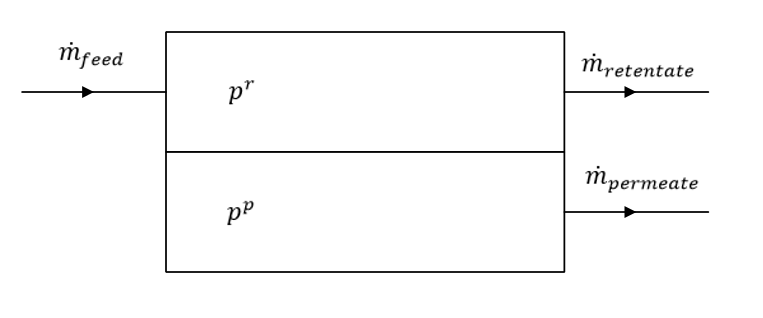
\includegraphics[width= 0.5\textwidth]{Images/mathematical_model2.png}
	\captionof{figure}{Schematic of the co-current flow in a membrane separator.}
	\label{fig:fig5}
\end{figure}
The feed with a specific mass flow frate $\dot{m}^f$ and composition enters the unit and is divided into two streams: $\dot{m}^p$ on the permeate side and $\dot{m}^r$ leaving on the retentate side. The flow is assumed to be ideal, frictionless, incompressible, isothermal and at constant velocity. The continuity and species continuity equations are presented in 1D Cartesian coordinates for the above assumptions. The continuity equation is defined as:
\begin{align}
	&& \frac{\partial \rho}{\partial t} + \frac{\partial (\rho u)}{\partial x} = 0
\end{align} 
Note that for an incompressible fluid the density of the individual species does not change. However, the density of the mixture can change due to permeation which influences the fluid composition and is computed at the end of each time step according to:
\begin{align}
	&&	\rho =  \frac{p}{R_uT} \sum_{k=1}^{N}X_k(MW)_k
\end{align}    

The species conservation equation at the retentate side is given by:
\begin{align}
&&\frac{\partial (\rho Y^r_k)}{\partial t} + \frac{\partial}{\partial x}  \left( \rho u Y^r_k\right)
= \frac{\partial}{\partial x}  \left( \rho D_k \ \frac{\partial Y^r_k }{\partial x}  \right) + \dot{w}_k
\label{eq:massbalance}
\end{align}

with $Y^r_k$ the mass fraction of specie k, $\rho$ the density of the mixture, u the velocity of the fluid, $D_k$ the diffusivity of specie k and $\dot{w}_k$ the source/sink term of specie k.
The sink term is defined as:
\begin{align}
&&	\dot{w}_k = -P_k \Big[p^rMW^r_{mix}Y^r_k-p^pMW^p_{mix}Y^p_k\Big]
\label{eq1}
\end{align}

With $P_k$ the permeability of specie k, $p^r$ and $p^p$ the pressure at retentate and permeate side respectively and $MW_{mix}$ the molar weight of the mixture. Replacing $Y_k^r$ by $Y_k^p$ and flipping the sign of the sink term in Equation \ref{eq1} gives the species conservation equation at the permeate side. \\

The stage cut $\theta$, is a parameter which gives information on the performance of the membrane and is defined as:
\begin{align}
	&&	\theta = 1- \frac{\dot{m}^r}{\dot{m}^f}
\end{align}

\subsection{Boundary conditions}
The following boundary conditions are applied to the problem described above:
\[
Permeate =\begin{cases}
x = 0 \ : \ \ u = 0\\
x = L \ : \ \frac{\partial Y_k}{\partial x} = 0 
\end{cases}
\] 
\[
Retentate =\begin{cases}
x = 0 \ : \ \ u = u_{in} \ , \ Y_k = Y_{k,in}\\
x = L \ : \ \frac{\partial Y_k}{\partial x} = 0 
\end{cases}
\] 
For the transient cases the feed fuel composition is a function of time, e.g. $Y_{in} = Y_{in}(t)$. \\ \\  There is no need for pressure boundary conditions due to the assumption of constant pressure at retentate and permeate side. 
\subsection{Numerical method}
The fully implicit method is used because of its superior stability. The implicit discretised form of Equation \ref{eq:massbalance} is given by:
\begin{align}
&&	a_P Y^r_{k,P} = a_W Y^r_{k,W} +  a_E Y^r_{k,E} + b
\end{align}
where 
\begin{align}
&& a_P = a_W + a_E + a_P^\circ + \Delta F 
\end{align} \\
with 
\begin{align}
&&	a_P^\circ = \frac{\rho_P^\circ \Delta x}{\Delta t}
\end{align}
and 
\begin{align}
&& b = \dot{w}_k \Delta x + a_P^\circ Y^{r, \circ}_{k,P}
\end{align} 
In the equations above the superscript $\circ$ refers to the value of the current time step.  
The neighbour coefficients for the internal nodes of this equation for the hybrid differencing scheme are as follows:
\begin{table}[H]
	\centering
	\begin{tabular}{|l|l|l|}
		\hline
		$a_W$     & $a_E$   & $\Delta F$ \\ \hline  \vspace{-0.3cm}
		& & \\
        $max\left[F_w, \left(D_w + \frac{F_w}{2}\right),0\right]$  & $max\left[-F_e, \left(D_e - \frac{F_e}{2}\right),0\right]$  & $F_e - F_w$  \\ \hline
	\end{tabular}
\end{table}
In the above expressions the values of $F$ and $D$ are calculated with the following formulae:
\begin{table}[H]
	\centering
	\begin{tabular}{|l|l|l|}
		\hline
		$Face$     & $w$   & $e$ \\ \hline  \vspace{-0.3cm}
		& & \\
		$F$  &$(\rho u)_w A_w$ & $(\rho u)_e A_e$ \\ \hline \vspace{-0.3cm}
		& & \\
		$D$  &$\frac{D_k}{\delta x_{WP}}A_w$ & $\frac{D_k}{\delta x_{PE}}A_e$ \\ \hline		
	\end{tabular}
\end{table}
Note that for a one-dimensional case the cell face area is equal to 1. \cite{Versteeg2007} \\
Special attention is needed for the boundary nodes. For the first node the coefficient $a_W$ is set to 0 and $a_E$ remains unchanged. The coefficient $a_P$ is computed as:
\begin{align}
&&	a_P =  max\left[F_w, \left(D_w + \frac{F_w}{2}\right),0\right] + a_E  + a^\circ_P + F_e - F_w
\end{align} 
The source term for the first node is:
\begin{align}
&& b = \dot{w}_k \Delta x + (max\left[F_w, \left(D_w + \frac{F_w}{2}\right),0\right] + a^\circ_P )\cdot Y_{k,in}	
\end{align}

For the last node the coefficient $a_E$ is set to 0 and $a_W$ remains unchanged. The coefficient $a_P$ is computed as:
\begin{align}
&&	a_P = a_W  + max\left[-F_e, \left(D_e - \frac{F_e}{2}\right),0\right] +  a^\circ_P + F_e - F_w
\end{align} 

At every time step the boundary condition $\frac{\partial Y_k}{\partial x}|_{x=L} = 0 $ is enforced.  

\subsection{Validation}
\subsubsection{The solver}
The solver and hybrid scheme are tested with a simple example from the book "An Introduction to Computational Fluid Dynamics" written by H.K. Versteeg and W. Malalasekera.\cite{Versteeg2007} The case conditions are as follows: \\

\textit{N = 5; L = 1; $\delta x = \frac{L}{N}$ = 0.2; u = 2.5 m/s; F = $\rho$u = 2.5; D = $\frac{\Gamma}{\delta x}$= $\frac{0.1}{0.2} = 0.5$; Pe = $\frac{F}{D} = 5$} \\
with boundary conditions: $\phi = 1$ at x = 0 and $\phi = 0$ at x = L.\\

The obtained matrix form of the equation set is
\[\hspace{2.5cm}
\left[\begin{array}{ccccc} 
3.5		& 0 	& 0  	& 0 	& 0   \\
-2.5	& 2.5	& 0		& 0		& 0   \\
0		& -2.5	& 2.5	& 0		& 0   \\
0		& 0		&-2.5	& 2.5	& 0   \\
0		& 0 	& 0		&-2.5	& 2.5 \\
\end{array}\right] 
\left[\begin{array}{c}  	
 \phi_1   \\
 \phi_2   \\
 \phi_3   \\
 \phi_4   \\
 \phi_5   \\
\end{array}\right] = 
\left[\begin{array}{c}  	
3.5   \\
0     \\
0     \\
0     \\
0     \\
\end{array}\right]\]

The solution obtained with the TDMA solver is:

\[\hspace{4.5cm} 
\left[\begin{array}{c}  	
\phi_1   \\
\phi_2   \\
\phi_3   \\
\phi_4   \\
\phi_5   \\
\end{array}\right] = 
\left[\begin{array}{c}  	
1      \\
1      \\
1      \\
1      \\
0.7143 \\
\end{array}\right]\]
which is exactly the same as the provided solution. 
\subsubsection{Model}
The code is validated by comparing with results from \hl{here source of pictures}.
The pressure on retentate and permeate are 4 and 0.4 bar respectively. The feed gas consists of mole percentages: \newline 
$H_2O=0.97$ $CO_2= 10.33$ $O_2 =1.54$ and $AR = 87.16  $. The total length is set to 1 m and divided over 200 control volumes such that $\Delta x = 0.005$. The time step is 0.5 and the simulation time is 200. The velocity must be high enough such that the flow is convection controlled rather than diffusion controlled. This also means that the cell P\'eclet number must be at least larger than 2. The density is set to 1 in equation:

\begin{equation}
\frac{\partial (\rho Y_k)}{\partial t} + \nabla \cdot \left( \rho u Y_k\right)
= \nabla \cdot \left( \rho D_k \ \left(\nabla \cdot Y_k\right) \right) + \dot{w_k}
\label{eq:massbalance2}
\end{equation}
Equation \ref{eq:massbalance2} has to be solved twice, once for the retentate and once for the permeate side.\\ 

In the original case the mass-flow rate was set to 15.4292 kg/h which is different from the massflow rate used as boundary conditions in this case (which is equal to 5400 kg/h). The reason for this choice is the fact that the equation must be convection controlled to produce reliable results. The formula is convection controlled when $Pe = \frac{\rho u}{\left(\Gamma/\partial x\right)} >2$. However, it is still possible to compare the  concentrations of both cases by looking at the same stage cut, which is a dimensionless parameter. The results are shown in  Table \ref{tab:table1}, Figure \ref{fig:fig1} and Figure \ref{fig:fig2}

\begin{table}[H]
\centering
    \caption{Caption}
    \label{tab:table1} 
\begin{tabular}{|l|l|l|l|l|l|}
\hline
                    & Farouck   & Case 1    & Case 2    & Case 3    & Case $3^*$\\\hline
$L$                 & 1         & 1         & 1         & 1         & 2         \\ \hline
$\Theta$            & 0.1598    & 0.1598    & 0.1598    & 0.1215    & 0.1598    \\ \hline
$P^r $              & 4         & 4         & 4         & 4         & 4         \\ \hline
$P^p $              & 0.4       & 0.4       & 0.4       & 0.4       & 0.4       \\ \hline
$\dot{m}$           & 15.4292   & 5400      & 3600      & 9000      & 9000      \\ \hline
$X^{r,in}_{H_2O}$   & 0.973272  & 0.973272  & 0.973272  & 0.973272  & 0.973272  \\ \hline
$X^{r,in}_{CO_2}$   & 10.329175 & 10.329175 & 10.329175 & 10.329175 & 10.329175 \\ \hline 
$X^{r,in}_{O_2}$    & 1.541694  & 1.541694  & 1.541694  & 1.541694  & 1.541694  \\ \hline
$X^{r,in}_{AR}$     & 87.155861 & 87.155861 & 87.155861 & 87.155861 & 87.155861 \\ \hline \hline
$X^{r,out}_{H_2O}$  & 0.269631  & 0.280611  &  0.280908 & 0.384081  & 0.279205  \\ \hline
$X^{r,out}_{CO_2}$  & 5         & 5.109224  & 5.107196  & 6.173649  & 5.098282  \\ \hline
$X^{r,out}_{O_2}$   & 1,594795  & 1.594100  & 1.593979  & 1.588198  & 1.594247  \\ \hline
$X^{r,out}_{AR}$    & 93.135571 & 93.016066 & 93.017917 & 91.854072 & 93.0282656\\ \hline \hline
$\Bar{X}^p_{H_2O}$  & 4.711435  & 4.543060  & 4.534002  & 5.192736  & 4.541872  \\ \hline
$\Bar{X}^p_{CO_2}$  & 38.640964 & 38.137105 & 38.137651 & 40.739224 & 38.102186 \\ \hline
$\Bar{X}^p_{O_2}$   & 1.259588  & 1.272995  & 1.272973  & 1.207574  & 1.273867  \\ \hline
$\Bar{X}^p_{AR}$    & 55.388010 & 56.046840 & 56.055374 & 52.860466 & 56.082075 \\ \hline
\end{tabular}
\end{table}

\begin{figure}[H]
\centering
	\begin{subfigure}[]
		\centering
		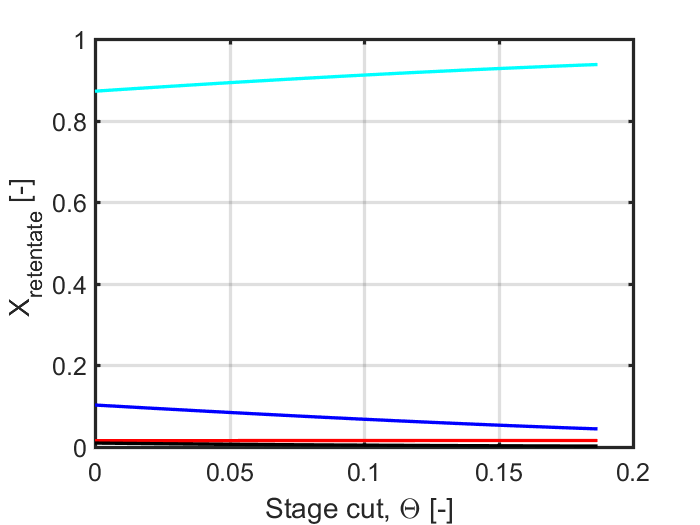
\includegraphics[width = 0.4\textwidth]{Images/x_retentate.png}
	\end{subfigure}
	\begin{subfigure}[]
		\centering
		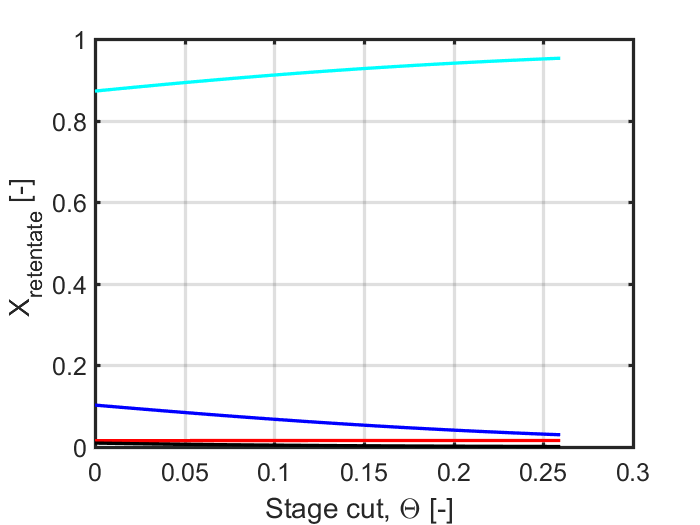
\includegraphics[width = 0.4\textwidth]{Images/x2_retentate.png}
	\end{subfigure}
	\begin{subfigure}[]
		\centering
		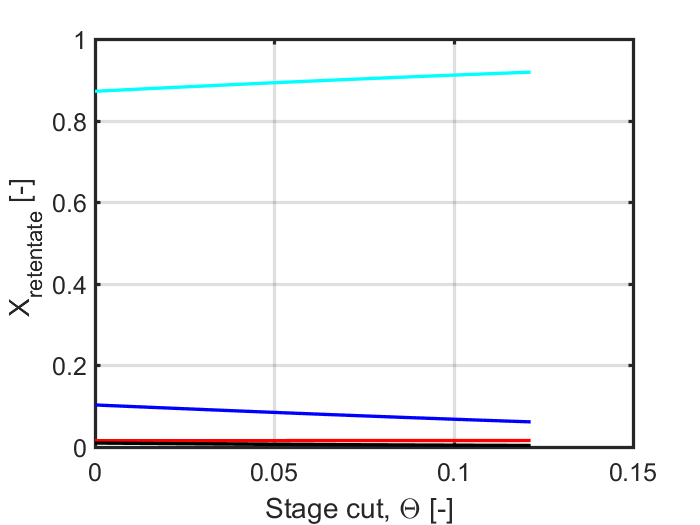
\includegraphics[width = 0.4\textwidth]{Images/x3_retentate.png}
	\end{subfigure}
	\begin{subfigure}[]
		\centering
		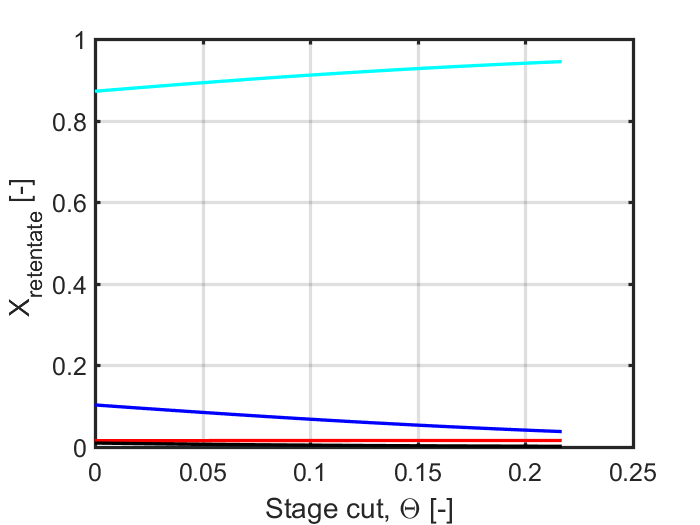
\includegraphics[width = 0.4\textwidth]{Images/x3star_retentate.png}
	\end{subfigure}	
\caption{a,b,c,d) $X^r$ for cases 1,2,3 and $3^*$ respectively }
\label{fig:fig1}
\end{figure}	

\begin{figure}[H]
\centering
	\begin{subfigure}[]
		\centering
		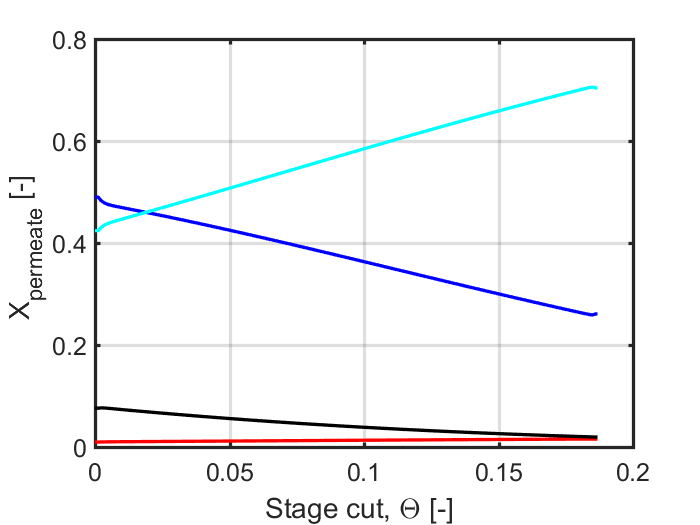
\includegraphics[width = 0.4\textwidth]{Images/x_permeate.png}
	\end{subfigure}
	\begin{subfigure}[]
		\centering
		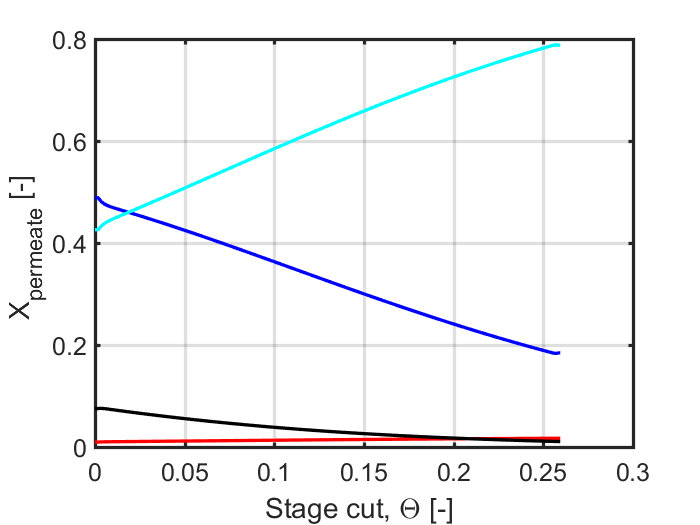
\includegraphics[width = 0.4\textwidth]{Images/x2_permeate.png}
	\end{subfigure}
	\begin{subfigure}[]
		\centering
		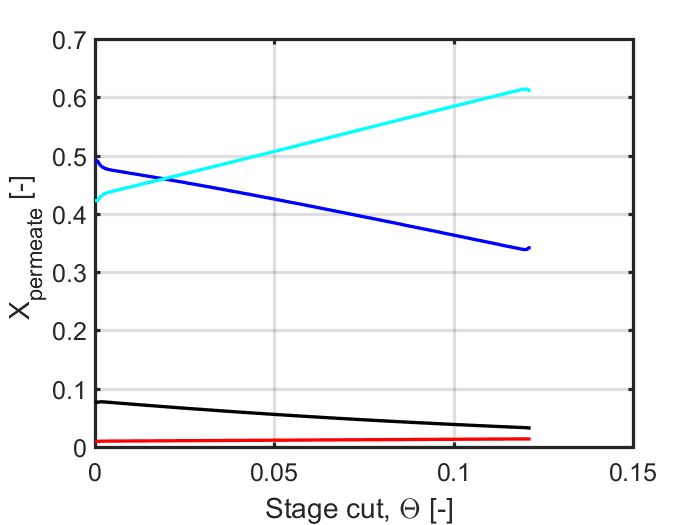
\includegraphics[width = 0.4\textwidth]{Images/x3_permeate.png}
	\end{subfigure}
	\begin{subfigure}[]
		\centering
		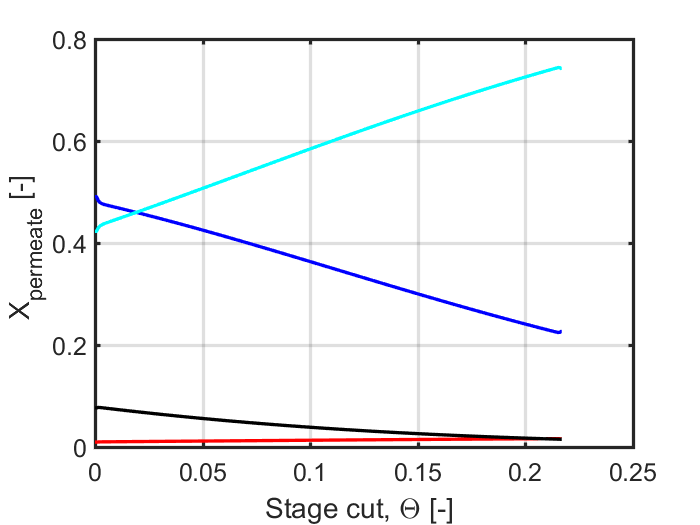
\includegraphics[width = 0.4\textwidth]{Images/x3star_permeate.png}
	\end{subfigure}	
\caption{a,b,c,d) $X^p$ for cases 1,2,3 and $3^*$ respectively }	
\label{fig:fig2}
\end{figure}

From the results it follows that at the same stage cut there is very little difference between the reference case (Faroucks results) and all other cases. Meaning that the velocity/ mass-flow rate has very little influence on the composition at a certain stage cut. However, the velocity does significantly influence the amount of membrane transport. In case 2, where the velocity is only 1 m/s and the mass-flow rate 3600 kg/h, the stage cut reaches a much larger value than for case 1 and 3. In case 3 the stage cut doesn't even reach the same value as the reference case. Hence, a second case 3 (case $3^*$) has been simulated with a length of 2 m instead of 1. 
\newpage

\section{Sensitivity}
A sensitivity analysis is performed on the pressure ratio and permeability of the species. First the results on the pressure ratio will be discussed. All results will be compared with a reference case, case 0, which has the following geometric and thermodynamic properties: \\ \\
The length of the domain is 1 meter and the grid is divided in 200 equal sized grid cells such that $\Delta x = 0.005$ meter. The inlet velocity is 1 m/s and remains constant. The temperature is 298 K and assumed to be constant over the entire domain, such that the flow can be regarded as isothermal. The total simulation time is 200 seconds and a time step of 0.05 seconds is used. The pressure at the retentate and permeate side are 400 and 40 kPa respectively, such that the pressure ratio is 0.1. The feed stream contains $X_{O_2}= 1.54 \%$, $X_{CO_2}= 10.33 \%$, $X_{H_2O}= 0.97 \%$ and $X_{AR}= 87.16 \%$. The permeability of $O_2$, $CO_2$, $H_2O$ and $AR$ are 28, 350, 1750 and 21 $\frac{n\ mol}{m \ s \ Pa}$ respectively\\ \\
 
\subsection{Pressure ratio}
\begin{table}[H]
\centering
\begin{tabular}{|l|l|l|l|l|}
\hline
                    & case 0    & case A1   & case A2 & case A3 \\ \hline
$\Theta$ \hspace{0.35cm}  [-]          & 0.261631  & 0.217092   & 0.116270 & 0.283972 \\ \hline
$P^r$   \hspace{0.35cm}  [Pa]          & 400       & 400       & 400     & 400     \\ \hline
$P^p$   \hspace{0.35cm}   [Pa]          & 40        & 80        & 200     & 20      \\ \hline \hline
$X^{r,out}_{H_2O}$ [-]  & 0.135988  & 0.135988  & 0.869079   & 0.021645        \\ \hline
$X^{r,out}_{CO_2}$ [-]  & 3.239114  & 5.728823  & 9.343992   & 1.848629        \\ \hline
$X^{r,out}_{O_2}$  [-]  & 1.593139  & 1.562543  & 1.535189   & 1.610194        \\ \hline
$X^{r,out}_{AR}$   [-]  & 95.031758 & 92.270670 & 88.251740  & 96.519533        \\ \hline
$X^{p}_{H_2O}$ \hspace{0.03cm}[-]  & 3.332514  & 3.075152  &  1.811850  &  2.942572       \\ \hline
$X^{p}_{CO_2}$ \hspace{0.03cm}[-]  & 31.952574 & 28.636889 & 18.284952  & 32.553121        \\ \hline
$X^{p}_{O_2}$  \ \ [-]  & 1.416297  & 1.467233  & 1.594041   &  1.422606       \\ \hline
$X^{p}_{AR}$  \hspace{0.06cm}   [-]  & 63.298615 & 66.820727 & 78.309158  &  63.081701       \\ \hline
\end{tabular}
\end{table}
From these results one can conclude that the concentration of species is quite sensitive to a change in pressure ratio. A lower pressure ratio results in more permeation and hence a larger value for the stage-cut and a decrease in concentration at the retenate side of species with a relative large permeability, as these species are most likely to permeate. Also, the mole fraction at the permeate side will increase for those species, due to the increase in permeation.\\
Comparing the reference case to cases with a larger pressure ratio shows that less species will permeate as the stage-cut decreases. As a consequence, the species with higher permeability will have a higher mole fraction at the retenate side and a lower mole fraction at the permeate side. For the species with a relative low permeability an increase of mole fraction is observed at the permeate side and a decrease at the retenate side. The change in mole fraction for the less permeating species is mainly because of the change in permeation of the species with a high permeability. The absolute value of species that has been permeated decreases for all species, no matter what the permeability is.
\begin{figure}[H]
\centering
	\begin{subfigure}[]
		\centering
		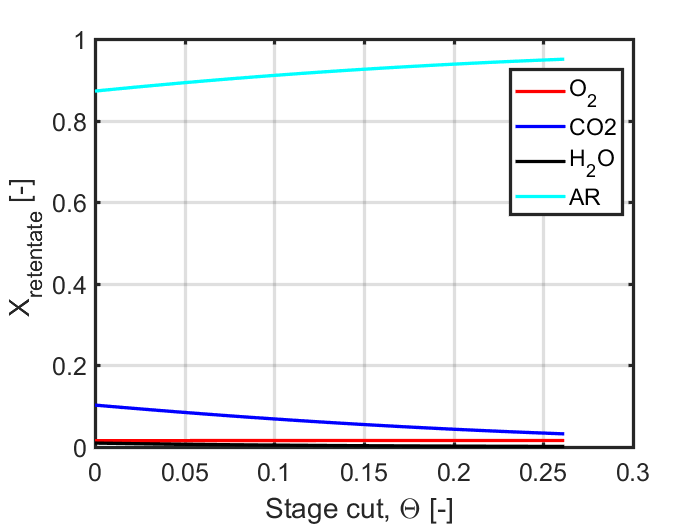
\includegraphics[width = 0.4\textwidth]{Images/case0_retenate.png}
	\end{subfigure}
	\begin{subfigure}[]
		\centering
		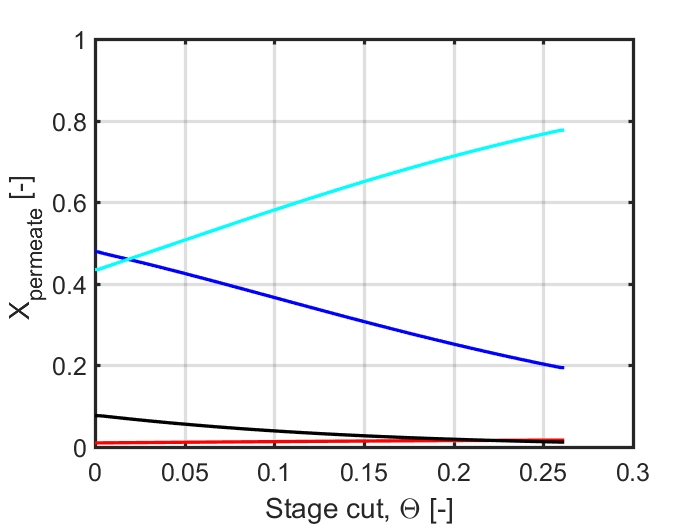
\includegraphics[width = 0.38\textwidth]{Images/case0_permeate.png}
	\end{subfigure}
	\begin{subfigure}[]
		\centering
		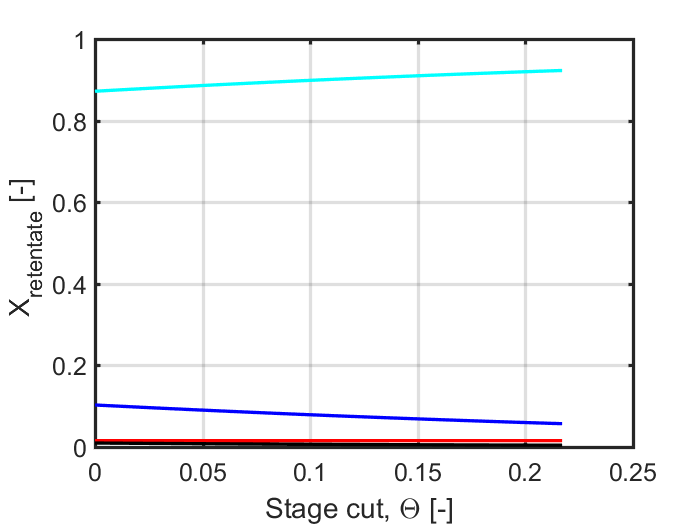
\includegraphics[width = 0.38\textwidth]{Images/case_A1_retenate.png}
	\end{subfigure}
	\begin{subfigure}[]
		\centering
	\end{subfigure}	
		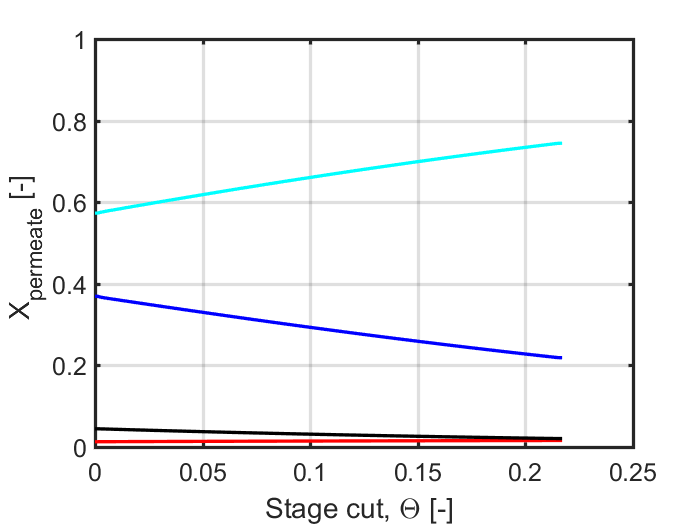
\includegraphics[width = 0.38\textwidth]{Images/case_A1_permeate.png}
	\begin{subfigure}[]
		\centering
		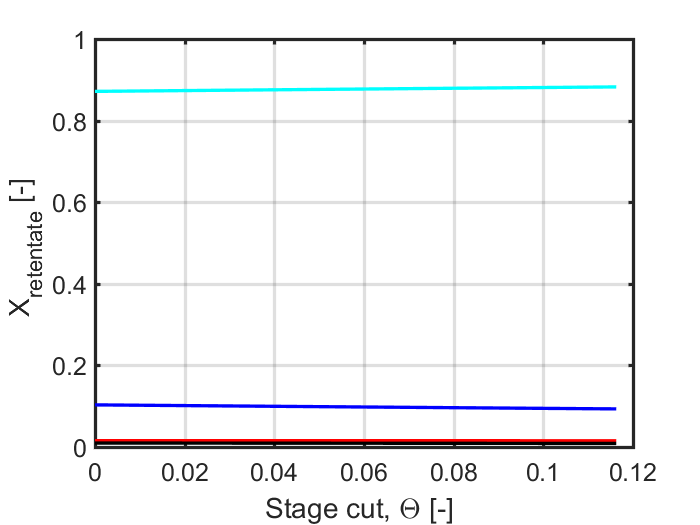
\includegraphics[width = 0.38\textwidth]{Images/case_A2_retenate.png}
	\end{subfigure}
	\begin{subfigure}[]
		\centering
		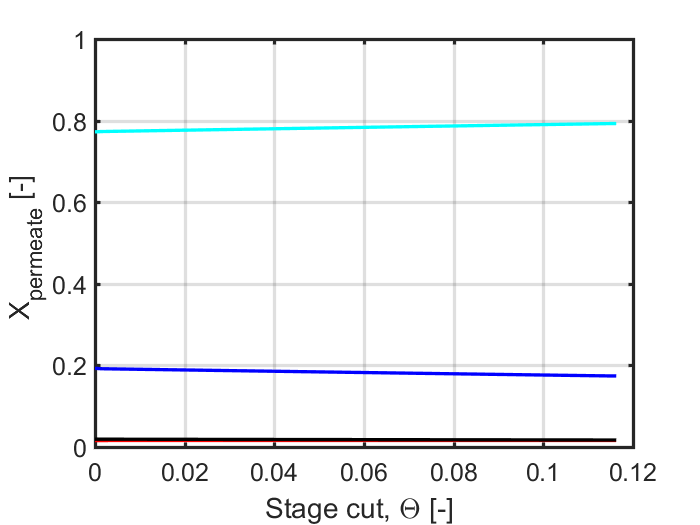
\includegraphics[width = 0.38\textwidth]{Images/case_A2_permeate.png}
	\end{subfigure}
	\begin{subfigure}[]
		\centering
		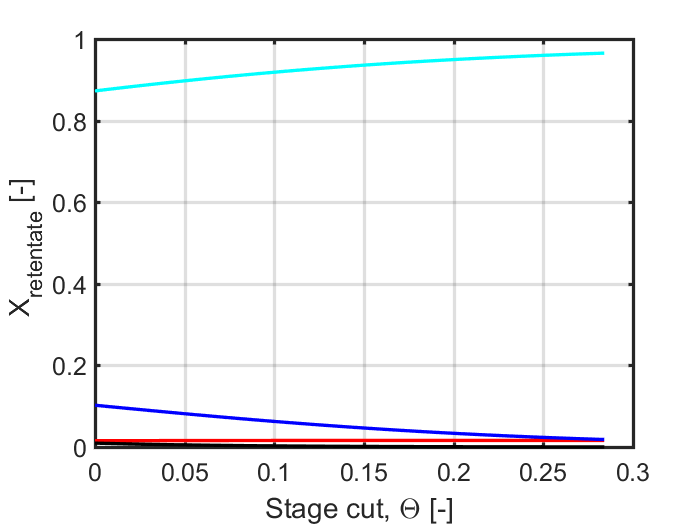
\includegraphics[width = 0.38\textwidth]{Images/case_A3_retenate.png}
	\end{subfigure}
	\begin{subfigure}[]
		\centering
		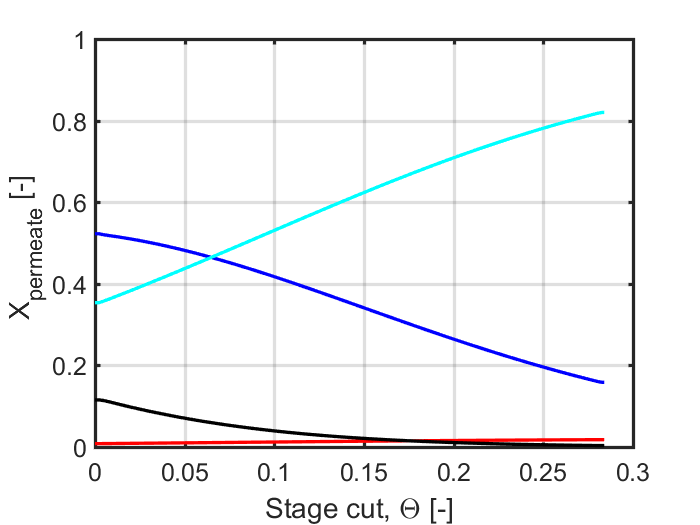
\includegraphics[width = 0.38\textwidth]{Images/case_A3_permeate.png}
	\end{subfigure}	
\caption{a,c,e,g) $X^r$ for cases 0, A1, A2 and A3 respectively. \newline b,d,f,h) $X^p$ for cases 0, A1, A2 and A3 respectively.}	
\label{fig:fig7}
\end{figure}

\subsection{Permeability}
This subsection treats the sensitivity of the species permeability. The permeability of only one species will be changed at the time. \\
Note that for better readability, the permeability in tables \ref{tab:table3}-\ref{tab:table6} is given in  $\frac{n\ mol}{m \ s \ Pa}$. 

\begin{table}[H]
\centering
\caption{Change in permeability of $H_2O$}
\label{tab:table3}
\begin{tabular}{|l|l|l|l|l|}
\hline
                    & case 0        & case B1       & case B2        \\ \hline
$\Theta$            & 0.261631      & 0.261339      & 0.261727       \\ \hline
$P_{H_2O}$          & 1750          & \textbf{875}  & \textbf{2625}  \\ \hline
$P_{CO_2}$          & 350           & 350           & 350            \\ \hline
$P_{O_2}$           & 28            & 28            & 28             \\ \hline
$P_{AR}$            & 21            & 21            & 21             \\ \hline \hline
$X^{r,out}_{H_2O}$  & 0.135988      & 0.179939      & 0.121488       \\ \hline
$X^{r,out}_{CO_2}$  & 3.239114      & 3.241211      & 3.238580       \\ \hline
$X^{r,out}_{O_2}$   & 1.593139      & 1.592407      & 1.593379       \\ \hline
$X^{r,out}_{AR}$    & 95.031758     & 94.986443     & 95.046554      \\ \hline
$X^{p}_{H_2O}$      & 3.332514      & 3.280739      & 3.341481       \\ \hline
$X^{p}_{CO_2}$      & 31.952574     & 32.019410     & 31.929929      \\ \hline
$X^{p}_{O_2}$       & 1.416297      & 1.416082      & 1.416550       \\ \hline
$X^{p}_{AR}$        & 63.298615     & 63.283768     & 63.312041      \\ \hline
\end{tabular}
\end{table}

\begin{table}[H]
\centering
\caption{Change in permeability of $CO_2$}
\label{tab:table4}
\begin{tabular}{|l|l|l|l|l|l|}
\hline
                    & case 0    & case C1   & case C2   & case C3  & case C4 \\ \hline
$\Theta$            & 0.261631  & 0.257586  & 0.219532  & 0.267289 & 0.272401\\ \hline
$P_{H_2O}$          & 1750      & 1750      & 1750      & 1750     & 1750    \\ \hline
$P_{CO_2}$          & 350       & \textbf{300}          & \textbf{100}     &\textbf{450} & \textbf{600}      \\ \hline
$P_{O_2}$           & 28        & 28        & 28        & 28        & 28   \\ \hline
$P_{AR}$            & 21        & 21        & 21        & 21        & 21   \\ \hline \hline
$X^{r,out}_{H_2O}$  & 0.135988  & 0.139131  & 0.175055  & 0.131866  & 0.128497   \\ \hline
$X^{r,out}_{CO_2}$  & 3.239114  & 3.594803  & 6.800644  & 2.734511  & 2.268858 \\ \hline
$X^{r,out}_{O_2}$   & 1.593139  & 1.587386  & 1.535971  & 1.601333  & 1.608944 \\ \hline
$X^{r,out}_{AR}$    & 95.031758 & 94.678680 & 91.488330 & 95.532290 & 95.993701\\ \hline
$X^{p}_{H_2O}$      & 3.332514  & 3.401261  & 3.960111  & 3.229445  & 3.126479 \\ \hline
$X^{p}_{CO_2}$      & 31.952574 & 31.511810 & 24.227410 & 32.364962 & 32.434709\\ \hline
$X^{p}_{O_2}$       & 1.416297  & 1.424700  & 1.571161  &  1.408974 &  1.408945\\ \hline
$X^{p}_{AR}$        & 63.298615 & 63.662229 & 70.241317 &  62.996620& 63.029867\\ \hline
\end{tabular}
\end{table}

\begin{table}[H]
\centering
\caption{Change in permeability of $O_2$}
\label{tab:table5}
\begin{tabular}{|l|l|l|l|l|}
\hline
                    & case 0        & case D1       & case D2       & case D3  \\ \hline
$\Theta$            & 0.261631      & 0.263137      & 0.259802      & 0.267235 \\ \hline
$P_{H_2O}$          & 1750          & 1750          & 1750          & 1750     \\ \hline
$P_{CO_2}$          & 350           & 350           & 350           & 350      \\ \hline
$P_{O_2}$           & 28            & \textbf{42}   & \textbf{14}   & \textbf{100} \\ \hline
$P_{AR}$            & 21            & 21            & 21        & 21        \\ \hline \hline
$X^{r,out}_{H_2O}$  & 0.135988      & 0.134462      & 0.137878  & 0.130443  \\ \hline
$X^{r,out}_{CO_2}$  & 3.239114      & 3.227465      & 3.253670  & 3.197499  \\ \hline
$X^{r,out}_{O_2}$   & 1.593139      & 1.443002      & 1.774387  & 1.029461  \\ \hline
$X^{r,out}_{AR}$    & 95.031758     & 95.195071     & 94.834065 & 95.642597 \\ \hline
$X^{p}_{H_2O}$      & 3.332514      & 3.314943      & 3.353014  & 3.262660  \\ \hline
$X^{p}_{CO_2}$      & 31.952574     & 31.806157     & 32.128574 & 31.396662 \\ \hline
$X^{p}_{O_2}$       & 1.416297      & 1.914029      & 0.793902  & 3.192724  \\ \hline
$X^{p}_{AR}$        & 63.298615     & 62.964871     & 63.724510 &  62.147954\\ \hline
\end{tabular}
\end{table}

\begin{table}[H]
\centering
\caption{Change in permeability of $AR$}
\label{tab:table6}
\begin{tabular}{|l|l|l|l|l|}
\hline
                    & case 0        & case E1       & case E2        \\ \hline
$\Theta$            & 0.261631      & 0.166233      & 0.350280       \\ \hline
$P_{H_2O}$          & 1750          & 1750          & 1750           \\ \hline
$P_{CO_2}$          & 350           & 350           & 350            \\ \hline
$P_{O_2}$           & 28            & 28            & 28             \\ \hline
$P_{AR}$            & 21            & \textbf{10.5} & \textbf{30.5}  \\ \hline \hline
$X^{r,out}_{H_2O}$  & 0.135988      & 0.259462      & 0.079392       \\ \hline
$X^{r,out}_{CO_2}$  & 3.239114      & 4.166193      & 2.793925       \\ \hline
$X^{r,out}_{O_2}$   & 1.593139      & 1.463864      & 1.127407       \\ \hline
$X^{r,out}_{AR}$    & 95.031758     & 94.110481     & 95.392418      \\ \hline
$X^{p}_{H_2O}$      & 3.332514      & 4.523370      & 2.652273       \\ \hline
$X^{p}_{CO_2}$      & 31.952574     & 42.510894    & 26.185366      \\ \hline
$X^{p}_{O_2}$       & 1.416297      & 2.041440      & 1.416550       \\ \hline
$X^{p}_{AR}$        & 63.298615     & 50.924295     & 70.034954     \\ \hline
\end{tabular}
\end{table}

From tables \ref{tab:table3}-\ref{tab:table6} one can conclude that the permeability can have a major influence on the permeation of species, but that the impact of the permeability also depends on the concentration of species. For instance, if there is only a small amount of a certain species there is not much to permeate even though the permeability might be relatively high, as is the case for $H_2O$ in Table \ref{tab:table3}. If on the other hand the permeability is relative small but the concentration of species is very high, then only a small difference in permeability can causes a big difference in concentration at the permeate side, see Table \ref{tab:table6}.  